\chapter{Anomaly Detection}

In data mining, \textit{Anomaly Detection} is a classification problem: the goal is finding patterns in data that do not conform to expected behavior \cite{chandola2009anomaly}. These patterns often denote an underlying different process: an anomaly can be defined an observation which deviates so much from the other observations as to arouse suspicions that it was generated by a different mechanism \cite{hawkins1980identification}.

This task finds extensive use in many domains, such as fraud detection for credit cards, insurance or health care, intrusion detection for cyber security, military surveillance and fault detection in critical systems.

Anomalies are also referred to as outliers, novelties, deviations, exceptions or noise. \textit{Noise removal} and \textit{noise accomodation} are related problems, dealing with the removal of unwanted objects before performing data analysis (removal) and immunizing a statistical model against anomalous observations (accomodation).

Methods make use of tools and concepts from a number of different fields, such as machine learning, data mining, information theory, spectral theory and statistics.

\subsection{Challenges}

Anomaly detection is an hard and complex problem, mainly due to the following challenging factors:

\begin{enumerate}
	\item Defining the normal and anomalous regions and their boundaries;
	\item The notion of \textit{normality} may evolve with time;
	\item Anomalies may be different for different domains; A small fluctuation might be significant in one domain while being a normal in another one;
	\item Availability and quality of labeled data;
	\item Noisy data and anomalies can be hard to discriminate.
\end{enumerate}

In practise, most techniques and approaches attack only a specific configuration (or formulation) of the problem.

Several factors determines this formulation formulation: nature of the datasets, availability of labeled instances, type of anomalies to detect.

\subsection{Nature of data}

The input is usually a collection of data instances (record, event, observation), described by one (univariate) or more (multivariate) attributes (feature, variable). Each attribute can be of different types (binary, categorical, continuos).


\subsection{Type of Anomaly}

\paragraph{Point Anomalies} The simplest scenario, when a single instance can be considered an anomaly in respect to the rest. E.g. in credit card fraud detection, a transaction for which the amount spent is very high compared to the normal range will be considered a point anomaly.

This type of anomalies can occur in any type of data set.

\paragraph{Contextual Anomalies} Given a notion of context in the problem formulation, a data instance can be considered anomalous in a specific context (but not otherwise). In this scenario, each data instance is defined with \textit{Contextual} and \textit{Behavioral} attributes. Contextual attributes define the context of that instance, e.g. \textit{longitude} and \textit{latitude} are contextual attributes in spatial data sets, while \textit{time} is a contextual attribute which determines the position of an instance in time series data. Behavioral attributes provide non-contextual information about the instance. E.g. the \textit{amount} of rainfall at any location.

Meaningfullness of the contextual anomalies in the target domain, availability of contextual attributes, feasability of defining a context are key factors in deciding which technique to apply.

Contextual anomalies have been explored in time-series and spatial data.

\paragraph{Collective Anomalies} If a subsequence of the dataset is anomalous with respect to the entire dataset, it is termed as collective anomaly. The individual instances making up the subsequence may not be anomalies by themselves, but their (ordered) occurence is anomalous. This type of anomalies requires the data instances to be related.

Sequence, spatial and graph datasets have been studied for this type of anomaly.

\begin{figure}
	\centerline{
		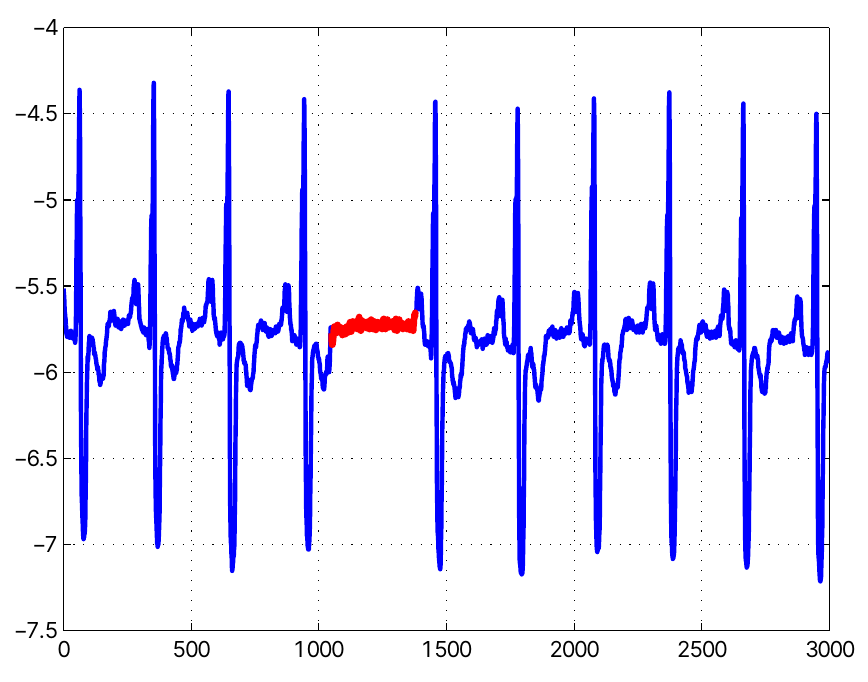
\includegraphics[width=0.4\paperwidth]{apc_ecg.png}}
	\caption{ Collective anomaly corresponding to an Atrial Premature Contraction in an human electrocardiogram output \cite{Goldberger2000PhysioBankPA} \cite{chandola2009anomaly}}
	\label{fig:apc_ecg}
\end{figure}


\subsection{Data labels}

The information associated with a data instance, describing if that instance is normal or anomalous is called labelling. Obtaining accurate and representative labelled data is often prohibitive expensive: it usually requires manual human effort, covering all possible scenarios of "anomalies" is expensive

Availability of labels influence the modality of the applicable anomaly detection techniques:

\subsubsection{Supervised}

In presence of training data with labeled data for both normal and anomaly class, this problem is similar to building predictive models for normal vs. anomaly classes.

Two issues can arise: \textit{imbalanced class distribution} and the non-triviliaty of \textit{obtaining accurate and significant labels} (especially for the anomaly class).


\subsubsection{Semi-supervised}

If training data has labeled instances for the normal class only, we resort to techniques operating in a semi-supervised mode, since they don't require labels for the anomaly class. The idea is to build a model for the normal behavior(s) and then use it to identify anomalous instances.

\subsubsection{Unsupervised}

This class includes the most widely applicable techniques, since they do not require any training data. Here, we assume that normal instances are more frequent than the anomalous ones. If this doesn't happen, an high false alarm rate is to be expected.


\subsubsection{Evaluation}

Here, we introduce some classification performance metrics used to set up a formal procedure to evaluate different approaches.

\begin{table}[]
	\centering
	\begin{tabular}{lllll}
		                                     &          &                                           &          & \\
		\multirow{2}{*}{}                    &          & \multicolumn{2}{l}{\textbf{Ground Truth}} &            \\
		                                     &          & Positive                                  & Negative & \\
		\multirow{2}{*}{\textbf{Prediction}} & Positive & TP                                        & FP       & \\
		                                     & Negative & FN                                        & TN       &
	\end{tabular}
	\caption{Confusion Matrix}
	\label{table:confusion_matrix}
\end{table}

Table \ref{table:confusion_matrix} explains the following quantities:

\begin{itemize}
	\item TP True Positives
	\item FP False Positives
	\item FN False Negatives
	\item TN True Negatives
\end{itemize}

Receiver Operating Characteristics (ROC) diagrams show a classifier performance plotting the False Positive Rates (FPR) against the True Positive Rates (TPR) of the classifier for a different thresholds. The idea is maximise the area under the ROC curve.

Intuitively, precision is the ability of the classifier not to label as positive a sample that is negative while recall is a measure of the ability of the classifier to find all the positive samples. \cite{scikit-learn}


\begin{equation}
	TPR = Recall = r = \frac{TP}{TP+FN}
\end{equation}

\begin{equation}
	FPR = \frac{FP}{FP+TN}
\end{equation}

\begin{equation}
	Precision = p = \frac{TP}{TP+FP}
\end{equation}

\begin{equation}
	Accuracy = \frac{TP+TN}{TP+TN+FP+FN}
\end{equation}

\begin{equation}
	Error = 1 - Accuracy
\end{equation}

Another metric is the F-measure, defined as follows:

\begin{equation}
	F_\beta = (1 + \beta^2) \cdot \frac{\mathrm{p} \cdot \mathrm{r}}{(\beta^2 \cdot \mathrm{p}) + \mathrm{r}}
\end{equation}

Where $\beta$ is a positive real chosen such that recall is considered $\beta$ times as important as precision. In the case $\beta = 1$, we have the $F_1$ score:

\begin{equation}
	F_1 = 2 \cdot \frac{\mathrm{p} \cdot \mathrm{r}}{\mathrm{p} + \mathrm{r}}
\end{equation}



\subsection{Output of Anomaly Detection}

Outputs produced by anomaly detection techniques can be Scores or Labels. In the case of anomaly scores \cite{chandola2009anomaly}, higher values indicate an higher probability that the data tuple is anomalous.


\subsection{Applications}


